\documentclass[paper=a5,10pt,openany]{scrbook}
\usepackage[footnotesep=1.5\baselineskip,twoside, top=0.06\paperheight, bottom=0.06\paperheight, left=0.125\paperwidth,
right=0.125\paperwidth, headsep=0.02\paperheight, foot=0.01\paperheight, bindingoffset=0\paperheight,heightrounded,includeheadfoot]{geometry}

\usepackage{background}

\parskip=0pt
\raggedbottom
\usepackage{opcdevocionario}%%Ficheiro sty na pasta controla os pacotes todos
\usepackage{tipografia}%%Ficheiro sty na pasta controla a tipografia

\setkomafont{subject}{\scshape}
\setkomafont{title}{\Huge}
\setkomafont{subtitle}{\scshape\color{red}}
\setkomafont{author}{\scshape}
\setkomafont{date}{\itshape\color{red}}

\setkomafont{chapter}{\normalfont\Large\scshape}
\renewcommand*{\raggedchapter}{\centering}

\begin{document}
\pagenumbering{gobble}% Remove page numbers (and reset to 1)
\backgroundsetup{scale=1,opacity=1,angle=0,position=current page.center,contents={
\includegraphics[width=1.1\textwidth, height=1.1\textheight]{frame6}}}

\begin{titlepage}
\begin{center}
\vspace*{2.5cm}
\Huge{Sanctum Rosarium}\\
\large{Santo Rosário}
\vspace*{1cm}

\includegraphics[width=0.85\textwidth]{sanctemichael}
\vspace*{1cm}
\Large{\redx Militia Sancti Michæli}\\
\large{2018}\\

\end{center}
\end{titlepage}

\sloppy%Justifica texto
\pretolerance=-1
\tolerance=3000
\adjdemerits=6400
\doublehyphendemerits=8000000
\finalhyphendemerits=14400
\hbadness=99999

\backgroundsetup{scale=1,opacity=1,angle=0,position=current page.center,contents={
\includegraphics[width=1.1\textwidth, height=1.1\textheight]{frame6}}}

\NewDocumentEnvironment{hangparacol}{mo}% LADO A LADO
  {\IfNoValueTF{#2} {\begin{paracol}{#1}}{\begin{paracol}{#1}[#2]}%
   \raggedright
   \parindent=3em \leftskip=3em}
  {\end{paracol}}
\columnratio{0.47}
\setlength{\columnseprule}{0pt}
\setlength{\columnsep}{3mm}
\colseprulecolor{red}

\pagenumbering{arabic}

\textbf{Católico:}

Colocamos nas suas mãos este livrinho, com a intenção de o ajudar a rezar o Santo Rosário de Nossa Senhora.

A oração do Santo Rosário é uma tradição milenar e deve o seu nome à ideia de que, ao rezar-se cada conta que o compõe, se oferece uma rosa à Mãe de Deus. Rosário, ou \textit{roseiral}, invoca, pois, a oferenda de uma flor preciosa, tão apreciada no Oriente e no Ocidente, a Nossa Senhora, Ela Própria invocada como \textit{Rosa Mystica.}

O Santo Rosário compreende três partes. Por este motivo, em Portugal, refere-se frequentemente o terço, para designar uma das três que compõem o conjunto, o qual tem 150 contas menores (por cada uma, a Ave Maria), divididas em dezenas e intercaladas por 15 contas maiores (por cada conta, o \textit{Pater Noster}), juntando-se-lhe a Ladainha da Santíssima Virgem (Lauretana) e outras orações, que o enriquecem, designadamente ao Sacratíssimo Coração de Nosso Senhor Jesus Cristo, a São Miguel Arcanjo e a São José. O número de contas menores alude aos 150 salmos, motivo pelo qual também se chamou Saltério de Nossa Senhora ao Santo Rosário.

O Santo Rosário é um tesouro. São tantas as indulgências que lhe foram concedidas pelos Papas que não podemos citá-las aqui. Para alcançá-las será necessário recitar todas as contas e meditar em cada mistério, com as condições habituais para lucrar indulgência: ter horror ao pecado, ir à Confissão e à Sagrada Comunhão, ambas com a intenção de obter a indulgência; e orações pelas Intenções do Santo Padre, as quais estão já agregadas ao Santo Rosário (as quatro contas que se seguem ao crucifixo).

Um rosário ou terço não é um objecto decorativo. Pela sua natureza devocional, dispensa cores berrantes e acrescentos mundanos, como missangas e outras quinquilharias, cujo uso chega a roçar a profanação. Opte por um rosário ou terço com forma tradicional e cores sóbrias (preto, branco, castanho, \&c.), cuja cruz apresente a imagem de Nosso Senhor Crucificado, podendo acrescentar-lhe uma medalha de Nossa Senhora. O seu rosário ou terço deve ser devidamente benzido por um sacerdote ou bispo. Depois desta bênção, é um sacramental. Por isso, beije-o, traga-o consigo, como quem traz uma jóia ou relíquia da Mãe de Deus; como quem está munido de uma arma poderosa, que usará para se defender do Inimigo.

Trazer o rosário ou terço consigo não bastará. É preciso que o reze, todos os dias, com muita devoção: diante do Santíssimo Sacramento, diante de uma imagem de Nossa Senhora, em igrejas, capelas, em casa, pela rua. Se esmorecer na oração, reze-o mesmo a contragosto e peça a Nossa Senhora que lhe melhore o ânimo. Procure rezar sem pressa, devagar, pronunciando bem cada palavra e sem se distrair com pensamentos inúteis.

Este livrinho está organizado em duas colunas: uma em latim – a língua que a Santa Igreja usa há séculos e que dedica, por excelência, ao Culto Divino – e em português. Poderá optar por rezar em qualquer uma das línguas ou por rezar apenas algumas partes em português.

Se possível, ponha-se de joelhos para rezar o Santo Rosário. Esta postura corporal e outros gestos são muito importantes, porque é certo que não rezamos apenas com a boca, mas com a totalidade do nosso corpo. Rezar de joelhos dispõe-nos a alma com humildade, diante da majestade de Deus, e corresponde certamente aos apelos de Nossa Senhora em Fátima: não veio pedir-nos apenas oração, mas também penitência. Com o Santo Rosário podemos peregrinar de joelhos pelos mistérios da vida de Nosso Senhor e da Santíssima Virgem, contemplando, em cada mistério, os episódios do Evangelho e os seus frutos, concedidos aos fiéis ao longo de tantos séculos.

Nas aparições de Fátima, a Santíssima Virgem apresentou-Se com o Seu título de Senhora do Rosário \textit{(Regina Sacratissimi Rosarii)} e pediu que rezássemos o terço todos os dias. Respondamos-Lhe com fidelidade, nas alegrias e nas tribulações da vida. Pelo Seu Santo Rosário caminharemos na conversão, pedindo perdão pelos nossos pecados, pedindo a conversão dos outros, desagravando o Sacratíssimo Coração de Nosso Senhor Jesus Cristo e o Imaculado Coração de Nossa Senhora. Podemos também suplicar por todas as nossas necessidades, implorar e agradecer milagres.

É muitíssimo poderosa a oração do Santo Rosário em família ou em grupos de amigos, mesmo pequenos. Procure, pois, expandir a devoção do Santo Rosário entre os seus familiares e amigos, oferendo-lhes um rosário ou um terço e, sobretudo, ensinando-os a rezá-lo. Se tiver avós ou tios idosos, peça-lhes que o ensinem a rezar o Santo Rosário, do modo como foram ensinados pelos respectivos pais e avós. Ensine os seus filhos, netos, sobrinhos e afilhados a rezá-lo. Lembre-se do exemplo dos Santos Pastorinhos: eram tão pequenos e foram tão fiéis aos pedidos do Céu. Por isso, alcançaram a santidade.

\textit{Laus Deo semper.}

Lisboa, Semana Santa de 2018


\textbf{Militia Sancti Michæli:}
\columnratio{0.55}
\begin{paracol}{2}
\small{
Aloisius, Miles Sancti Aloisii Mariæ Grignion

Aloisius, Miles Sancti Ioannis Fisher

Alphonsus, Miles Sancti Pii X

Bernardus, Miles Sanctæ Hyacinthæ

Emanuel, Miles Sancti Nonii de Sancta Maria

Emanuel, Miles Sancti Pauli

Didacus, Miles Sancti Francisci Salesii

Ferdinandus, Miles Sanctæ Crucis

Georgius, Miles Sancti Ioseph

Helder, Miles Sancti Patris Pii

Hubertus, Miles Sancti Pii V

Ioannes, Miles Sancti Petri

Ioannes, Miles Sancti Ioannis Baptista

Ioseph, Miles Sancti Antonius Olisiponensis

Ioseph, Miles Sanctæ Catharinæ Senensis

Ioseph, Miles Sanctæ Mariæ

Michæl, Miles Sancti Fratris Ægidii

Michæl, Miles Sanctæ Mariæ Magdalenæ

Michæl, Miles Sancti Nicolai
\switchcolumn
Marcus, Miles Sancti Gregorii Pauli

Nonius, Miles Sancti Nonii de Sancta Maria

Petrus, Miles Sancti Gregorii

Simon, Miles Sancti Athanasii
}
\end{paracol}

\newpage

\section{Sanctum Rosarium}
\columnratio{0.47}
\begin{nscenter}Santo Rosário\end{nscenter}

\emph{\redx{Ajoelhe-se. Segure devotamente o crucifixo do seu rosário ou terço e beije-o. Com o crucifixo, faça o Sinal da Santa Cruz.}}

\subsubsection{Signum Crucis - Sinal da Cruz}
\begin{paracol}{2}
\cruz In nómine Patris, et Fílii, et Spíritus Sancti.
\switchcolumn
\cruz Em nome do Pai e do Filho e do Espírito Santo.
\switchcolumn*
℟. Amen.
\switchcolumn
℟. Amen.
\end{paracol}

\emph{\redx{Com o crucifixo erguido nas mãos, reze as orações que se seguem.}}

\subsection{Ad Crucem}
\begin{nscenter}No Crucifixo\end{nscenter}
\subsubsection{Symbolum Apostolorum - Símbolo dos Apóstolos}
\begin{paracol}{2}
\blettrine{C}{redo} in Deum, Patrem omnipoténtem, Creatórem cæli et terræ. Et in Jesum Christum, Fílium eius únicum, Dóminùm nostrum: qui concéptus est de Spíritu Sancto, natus ex María Vírgine, passus sub Pontio Piláto, crucifíxus, mórtuus, et sepúltus: descéndit ad ínferos; tértia die resurréxit a mórtuis; ascéndit ad cælos; sedet ad déxteram Dei Patris omnipoténtis: inde ventúrus est judicáre vivos et mórtuos. Credo in Spíritum Sanctum, sanctam Ecclésiam cathólicam, Sanctórum communionem, remissiónem peccatórum, carnis resurrectiónem, vitam ætérnam.
\switchcolumn
\blettrine{C}{reio} em Deus, Pai todo-poderoso, Criador do Céu e da Terra; e em Jesus Cristo, seu único Filho, Nosso Senhor, que foi concebido pelo poder do Espírito Santo; nasceu da Virgem Maria; padeceu sob Pôncio Pilatos, foi crucificado, morto e sepultado; desceu à mansão dos mortos; ressuscitou ao terceiro dia; subiu aos Céus, onde está sentado à direita de Deus Pai todo-poderoso, de onde há-de vir a julgar os vivos e os mortos. Creio no Espírito Santo, na santa Igreja Católica; na comunhão dos Santos; na remissão dos pecados; na ressurreição da carne; na vida eterna.
\switchcolumn*
℟. Amen.
\switchcolumn
℟. Amen.
\end{paracol}

\pagebreak [3]

\subsubsection{Confiteor - Confesso}

\emph{\redx{Incline o corpo para a frente, dobre a cabeça para baixo e reze o seguinte:}}

\begin{paracol}{2}
\rlettrine{C}{onfíteor} Deo omnipoténti, beátæ Maríæ semper Vírgini, beáto Michǽli Archángelo, beáto Joánni Baptístæ, sanctis Apóstolis Petro et Paulo, ómnibus Sanctis, et tibi, pater: quia peccávi nimis cogitatióne, verbo et ópere: \emph{(Percutit sibi pectus ter, dicens:)}
\switchcolumn
\rlettrine{E}{u} me confesso a Deus, todo poderoso, à bem-aventurada sempre Virgem Maria, ao bem-aventurado S. Miguel Arcanjo, ao bem-aventurado S. João Baptista, aos Santos Apóstolos S. Pedro e S. Paulo, a todos os santos, e a vós, Padre: que pequei muitas vezes por pensamentos, palavras e obras: \emph{(Feche a mão direita e bata no peito por três vezes.)}
\switchcolumn*
\begin{nscenter}\emph{\redx{Mea culpa, mea culpa, mea máxima culpa.}}\end{nscenter}
\switchcolumn
\begin{nscenter}\emph{\redx{Por minha culpa, por minha culpa, por minha tão grande culpa.}}\end{nscenter}
\switchcolumn*
Ideo precor beátam Maríam semper Vírginem, beátum Michǽlem Archángelum, beátum Joánnem Baptístam, sanctos Apóstolos Petrum et Paulum, omnes Sanctos, et te, pater, orare pro me ad Dóminum, Deum nostrum.
\switchcolumn
Portanto rogo à bem-aventurada sempre Virgem Maria, ao bem-aventurado S. Miguel Arcanjo, ao bem-aventurado S. João Baptista, aos Santos Apóstolos S. Pedro e S. Paulo, a todos os Santos e a vós, Padre, que rogueis a Deus, nosso Senhor, por mim.
\end{paracol}

\subsubsection{Oferecimento do Santo Rosário}

\rlettrine{S}{antíssima} Virgem, Mãe de Deus, eu Vos ofereço este rosário em desagravo do Santíssimo Coração de Nosso Senhor Jesus Cristo, Vosso Filho, e em desagravo do Vosso Coração Imaculado; e pelas intenções que Vos apresento: \emph{(Referir as intenções.)}

\emph{\redx{Em seguida, anuncie que as orações depois do crucifixo serão rezadas pelas Intenções do Santo Padre.}}

\subsubsection{Intenções do Santo Padre}
\begin{paracol}{2}
\begin{compactitem}
\item Exaltatio S. Matris Ecclesiæ.
\switchcolumn
\item Exaltação da Santa Igreja.
\switchcolumn*
\item Propagatio fidei.
\switchcolumn
\item Propagação da fé.
\switchcolumn*
\item Extirpatio hæresum.
\switchcolumn
\item Extirpação das heresias.
\switchcolumn*
\item Conversio peccatorum.
\switchcolumn
\item Conversão dos pecadores.
\switchcolumn*
\item Pax inter principes christianos.
\switchcolumn
\item Paz entre os Reis e Príncipes católicos.
\end{compactitem}
\end{paracol}

\emph{\redx{Siga pela primeira conta, depois do crucifixo. Reze nela o Pater Noster. Siga pelas três contas seguintes. Reze em cada uma a Ave Maria. No final destas orações, reze a Glória (não tem conta). A conta seguinte corresponde ao Pater Noster do primeiro mistério.:}}

\subsection{Ad Grana Maiora}
\begin{nscenter}Nas contas maiores\end{nscenter}
\subsubsection{Pater Noster - Pai Nosso}
\begin{paracol}{2}
℣. Pater noster, qui es in cælis: sanctificétur nomen tuum: advéniat regnum tuum: fiat volúntas tua, sicut in cælo, et in terra.
\switchcolumn
℣.Pai Nosso, que estais nos céus, santificado seja o Vosso Nome, venha a nós o Vosso Reino; seja feita a Vossa vontade assim na terra como no Céu.
\switchcolumn*
℟. Panem nostrum quotidiánum da nobis hódie: et dimítte nobis débita nostra, sicut et nos dimíttimus debitóribus nostris. Et ne nos indúcas in tentatiónem. Sed líbera nos a malo.
\switchcolumn
℟. O pão nosso de cada dia nos dai hoje; perdoai-nos as nossas ofensas, assim como nós perdoamos a quem nos tem ofendido; e não nos deixeis cair em tentação; mas livrai-nos do mal.
\switchcolumn*
℟. Amen.
\switchcolumn
℟. Amen.
\end{paracol}

\subsection{Ad Grana Minora}
\begin{nscenter}Nas contas menores\end{nscenter}
\subsubsection{Ave Maria}
\begin{paracol}{2}
℣.Ave, María, grátia plena, Dóminus tecum; benedícta tu in muliéribus, et benedíctus fructus ventris tui, Jesus.
\switchcolumn
℣.Ave, Maria, Cheia de graça, o Senhor é convosco; bendita sois Vós entre as mulheres, e bendito é o fruto do Vosso ventre, Jesus.
\switchcolumn*
℟. Sancta María, Mater Dei, ora pro nobis peccatóribus, nunc, et in hora mortis nostræ.
\switchcolumn
℟. Santa Maria, Mãe de Deus, rogai por nós, pecadores, agora e na hora da nossa morte.
\switchcolumn*
℟. Amen.
\switchcolumn
℟. Amen.
\end{paracol}

\subsection{Ad Finem Decadum}
\begin{nscenter}No fim das dezenas\end{nscenter}
\subsubsection{Glória}
\begin{paracol}{2}
℣. Glória Patri, et Fílio, et Spíritui Sancto.
\switchcolumn
℣. Glória ao Pai, e ao Filho e ao Espírito Santo.
\switchcolumn*
℟. Sicut erat in pricípio, et nunc, et semper, et in sǽcula sæculórum.
\switchcolumn
℟. Assim como era no princípio, agora e sempre, e por todos os séculos dos
séculos.
\switchcolumn*
℟. Amen.
\switchcolumn
℟. Amen.
\end{paracol}

\subsubsection{Nossa Senhora a Santa Catarina Labouré}
\begin{paracol}{2}
℣. O Maria sine labe concepta.
\switchcolumn
℣. Ó Maria concebida sem pecado.
\switchcolumn*
℟. Ora pro nobis, qui confugimus ad te.
\switchcolumn
℟. Rogai por nós que recorremos a vós.
\end{paracol}

\subsubsection{Nossa Senhora aos Santos Pastorinhos}

\begin{paracol}{2}
℣. Oh mi Jesu, dimitte nobis débita nostra, líbera nos ab igne inférni,
\switchcolumn
℣. Ó meu Jesus, perdoai-nos e livrai-nos do fogo do inferno,
\switchcolumn*
℟. Conduc in cælum omnes animas, præsértim illas quæ máxime indigent
misericórdia tua.
\switchcolumn
℟. Levai as alminhas todas para o Céu e socorrei principalmente as que mais
precisarem.
\end{paracol}

\subsection{Meditationes Rosarii}
\begin{nscenter}Meditações do Rosário\end{nscenter}
\subsubsection{Mystéria Gaudiósa}
\begin{nscenter}Mistérios Gozosos\end{nscenter}
\begin{nscenter}\emph{\redx{Segunda-feira e Quinta-feira}}\end{nscenter}

{\redx Primeiro mistério:} Meditemos na Anunciação do Arcanjo São Gabriel à Santíssima Virgem, e roguemos a virtude da humildade.\par
{\redx Segundo mistério:} Meditemos na Visitação da Santíssima Virgem a Sua Prima, Santa Isabel, e roguemos a caridade para com o próximo.\par
{\redx Terceiro mistério:} Meditemos no Nascimento do Menino Jesus, e roguemos o desprendimento dos bens do mundo.\par
{\redx Quarto mistério:} Meditemos na Apresentação do Menino Jesus no Templo e na Purificação de Nossa Senhora, e roguemos a obediência e a pureza do espírito e do coração.\par
{\redx Quinto mistério:} Meditemos na Perda e no Encontro do Menino Jesus no Templo, e roguemos o conhecimento das coisas divinas e a prontidão no serviço de Deus.

\subsubsection{Mystéria Dolorósa}
\begin{nscenter}Mistérios Dolorosos\end{nscenter}
\begin{nscenter}\emph{\redx{Terça-feira e Sexta-feira}}\end{nscenter}

{\redx Primeiro mistério:} Meditemos na Agonia de N. S. Jesus Cristo, e roguemos a contrição dos nossos pecados.\par
{\redx Segundo mistério:} Meditemos na flagelação de N. S. Jesus Cristo, e roguemos a mortificação dos sentidos.\par
{\redx Terceiro mistério:} Meditemos na Coroação de Espinhos de N. S. Jesus Cristo, e roguemos a mortificação do espírito e do coração.\par
{\redx Quarto mistério:} Meditemos em N. S. Jesus Cristo levando a Cruz para o Calvário, e roguemos a paciência e a resignação.\par
{\redx Quinto mistério:} Meditemos na Crucifixão e Morte de N. S. Jesus Cristo, e roguemos o amor a Deus e a salvação das almas.

\subsubsection{Mystéria Gloriósa}
\begin{nscenter}Mistérios Gloriosos\end{nscenter}
\begin{nscenter}\emph{\redx{Quarta-feira, Sábado e Domingo}}\end{nscenter}

{\redx Primeiro mistério:} Meditemos na Ressurreição de N. S. Jesus Cristo, e roguemos para recebermos o dom da fé e para a conversão dos pecadores.\par
{\redx Segundo mistério:} Meditemos na Ascensão de N. S. Jesus Cristo, e roguemos a esperança e o desejo do céu.\par
{\redx Terceiro mistério:} Meditemos na descida do Divino Espírito Santo, e roguemos o amor a Deus e o zelo da salvação das almas.\par
{\redx Quarto mistério:} Meditemos na Assunção da Santíssima Virgem, e roguemos a graça de uma boa morte e a devoção a Nossa Senhora.\par
{\redx Quinto mistério:} Meditemos na Coroação da Santíssima Virgem, e roguemos a perseverança final e a confiança em Nossa Senhora.

\subsection{Orationes ad Finem Rosarii}
\begin{nscenter}Orações no fim do Rosário\end{nscenter}

\subsubsection{Salve Regina - Salve Rainha}
\begin{paracol}{2}
\blettrine{S}{alve,} Regina, Mater misericórdiæ, vita, dulcédo et spes nostra, salve. Ad te clamámus, éxsules fílii Hevæ. Ad te suspirámus geméntes et flentes in hac lacrimárum valle. Éia ergo, advocáta nostra, illos tuos misericórdes óculos ad nos convérte. Et Jesum benedíctum fructum ventris tui, nobis, post hoc exsílium, osténde. O clemens, o pia, o dulcis Virgo Maria!
\switchcolumn
\blettrine{S}{alvé,} Rainha, mãe de misericórdia, vida, doçura, esperança nossa, salve! A Vós bradamos, os degredados filhos de Eva. A Vós suspiramos, gemendo e chorando neste vale de lágrimas. Eia, pois, advogada nossa, esses Vossos olhos misericordiosos a nós volvei. E, depois deste desterro, nos mostrai Jesus, bendito fruto do Vosso ventre. Ó clemente, ó piedosa, ó doce Virgem Maria.
\switchcolumn*
℣. Ora pro nobis, Regina Sacratíssimi Rosárii.
\switchcolumn
℣. Rogai por nós, Rainha do Santíssimo Rosário.
\switchcolumn*
℟. Ut digni efficiámur promissiónibus Christi.
\switchcolumn
℟. Para que sejamos dignos das promessas de Cristo.
\switchcolumn*
\begin{nscenter} {\redx Orémus.} \end{nscenter}
\switchcolumn
\begin{nscenter} {\redx Oremos.} \end{nscenter}
\switchcolumn*
\rlettrine{D}{eus,} cujus Unigénitus per vitam, mortem et resurrectiónem suam nobis salútis ætérnæ prǽmia comparávit, concede, quǽsumus: ut hæc mystéria sacratissimo beátæ Maríæ Vírginis Rosário recoléntes, et imitémur quod continent, et quod promittunt assequámur. Per eundem Christum Dóminum
nostrum.
\switchcolumn
\slettrine{Ó}{} Deus, cujo Filho Unigénito por sua vida, morte e ressurreição nos alcançou os prémios da vida eterna, concedei-nos, Vos suplicamos, que, venerando nós estes mistérios do Santíssimo Rosário da Virgem Maria, imitemos o que eles contêm, e alcancemos o que eles prometem. Pelo mesmo Cristo, nosso Senhor.
\switchcolumn*
℟. Amen.
\switchcolumn
℟. Amen.
\end{paracol}

\newpage\begin{nscenter}
\includegraphics[width=1\textwidth,height=1\textheight,keepaspectratio]{anunciacao}
\end{nscenter}

\subsubsection{Litaniæ Lauretanæ Beatæ Mariæ Virginis}
\begin{nscenter}Ladainha da Santíssima Virgem\end{nscenter}

\begin{paracol}{2}
Kyrie, eléison.
\switchcolumn
Senhor, tende piedade de nós.
\switchcolumn*
Christe, eléison.
\switchcolumn
Jesus Cristo, tende piedade de nós.
\switchcolumn*
Kyrie, eléison.
\switchcolumn
Senhor, tende piedade de nós.
\switchcolumn*
Christe, áudi nos.
\switchcolumn
Jesus Cristo, ouvi-nos.
\switchcolumn*
Christe, exáudi nos.
\switchcolumn
Jesus Cristo, atendei-nos.
\switchcolumn*
Pater de cælis, Deus, miserére nobis.
\switchcolumn
Pai do Céu, que sois Deus, tende piedade de nós.
\switchcolumn*
Fili, Redémptor mundi, Deus,
\switchcolumn
Filho Redentor do mundo, que sois Deus,
\switchcolumn*
Spíritus Sancte, Deus,
\switchcolumn
Espírito Santo, que sois Deus,
\switchcolumn*
Sancta Trínitas, unus Deus,
\switchcolumn
Santíssima Trindade, que sois um só Deus,
\switchcolumn*
Sancta Maria, ora pro nobis.
\switchcolumn
Santa Maria, rogai por nós.
\switchcolumn*
Sancta Dei Génitrix,\footnote[2]{ora pro nobis.\label{ora}}
\switchcolumn
Santa Mãe de Deus,\footnote[2]{rogai por nós.\label{rogai}}
\switchcolumn*
Sancta Virgo vírginum,\footref{ora}
\switchcolumn
Santa Virgem das Virgens,\footref{rogai}
\switchcolumn*
Mater Christi,\footref{ora}
\switchcolumn
Mãe de Cristo,\footref{rogai}
\switchcolumn*
Mater Ecclésiæ,\footref{ora}
\switchcolumn
Mãe da Igreja,\footref{rogai}
\switchcolumn*
Mater divínæ grátiæ,\footref{ora}
\switchcolumn
Mãe da divina graça,\footref{rogai}
\switchcolumn*
Mater puríssima,\footref{ora}
\switchcolumn
Mãe puríssima,\footref{rogai}
\switchcolumn*
Mater castíssima,\footref{ora}
\switchcolumn
Mãe castíssima,\footref{rogai}
\switchcolumn*
Mater invioláta,\footref{ora}
\switchcolumn
Mãe imaculada,\footref{rogai}
\switchcolumn*
Mater intemeráta\footref{ora}
\switchcolumn
Mãe intacta,\footref{rogai}
\switchcolumn*
Mater amábilis,\footref{ora}
\switchcolumn
Mãe amável,\footref{rogai}
\switchcolumn*
Mater admirábilis,\footref{ora}
\switchcolumn
Mãe admirável,\footref{rogai}
\switchcolumn*
Mater boni consílii,\footref{ora}
\switchcolumn
Mãe do bom conselho,\footref{rogai}
\switchcolumn*
Mater Creatóris,\footref{ora}
\switchcolumn
Mãe do Criador,\footref{rogai}
\switchcolumn*
Mater Salvatóris,\footref{ora}
\switchcolumn
Mãe do Salvador,\footref{rogai}
\switchcolumn*
Virgo prudentíssima,\footref{ora}
\switchcolumn
Virgem prudentíssima,\footref{rogai}
\switchcolumn*
Virgo veneranda,\footref{ora}
\switchcolumn
Virgem venerável,\footref{rogai}
\switchcolumn*
Virgo prædicánda,\footref{ora}
\switchcolumn
Virgem louvável,\footref{rogai}
\switchcolumn*
Virgo potens,\footref{ora}
\switchcolumn
Virgem poderosa,\footref{rogai}
\switchcolumn*
Virgo clemens,\footref{ora}
\switchcolumn
Virgem clemente,\footref{rogai}
\switchcolumn*
Virgo fidélis,\footref{ora}
\switchcolumn
Virgem fiel,\footref{rogai}
\switchcolumn*
Speculum justitiæ,\footref{ora}
\switchcolumn
Espelho de justiça,\footref{rogai}
\switchcolumn*
Sedes sapiéntiæ,\footref{ora}
\switchcolumn
Sede de sabedoria,\footref{rogai}
\switchcolumn*
Causa nostræ lætítiæ,\footref{ora}
\switchcolumn
Causa da nossa alegria,\footref{rogai}
\switchcolumn*
Vas spirituále,\footref{ora}
\switchcolumn
Vaso espiritual,\footref{rogai}
\switchcolumn*
Vas honorábile,\footref{ora}
\switchcolumn
Vaso honorífico,\footref{rogai}
\switchcolumn*
Vas insígne devotiónis,\footref{ora}
\switchcolumn
Vaso insigne de devoção,\footref{rogai}
\switchcolumn*
Rosa mystica,\footref{ora}
\switchcolumn
Rosa mística,\footref{rogai}
\switchcolumn*
Turris davídica,\footref{ora}
\switchcolumn
Torre de David,\footref{rogai}
\switchcolumn*
Turris ebúrnea,\footref{ora}
\switchcolumn
Torre de marfim,\footref{rogai}
\switchcolumn*
Domus áurea,\footref{ora}
\switchcolumn
Casa de ouro,\footref{rogai}
\switchcolumn*
Fœderis arca,\footref{ora}
\switchcolumn
Arca da Aliança,\footref{rogai}
\switchcolumn*
Jánua cæli,\footref{ora}
\switchcolumn
Porta do Céu,\footref{rogai}
\switchcolumn*
Stella matutína,\footref{ora}
\switchcolumn
Estrela da manhã,\footref{rogai}
\switchcolumn*
Salus infirmórum,\footref{ora}
\switchcolumn
Saúde dos enfermos,\footref{rogai}
\switchcolumn*
Refúgium peccatórum,\footref{ora}
\switchcolumn
Refúgio dos pecadores,\footref{rogai}
\switchcolumn*
Consolátrix afflictórum,\footref{ora}
\switchcolumn
Consoladora dos aflitos,\footref{rogai}
\switchcolumn*
Auxílium christianórum,\footref{ora}
\switchcolumn
Auxílio dos cristãos,\footref{rogai}
\switchcolumn*
Regína angelórum,\footref{ora}
\switchcolumn
Rainha dos Anjos,\footref{rogai}
\switchcolumn*
Regína patriarchárum,\footref{ora}
\switchcolumn
Rainha dos Patriarcas,\footref{rogai}
\switchcolumn*
Regína prophetárum,\footref{ora}
\switchcolumn
Rainha dos Profetas,\footref{rogai}
\switchcolumn*
Regína apostolórum,\footref{ora}
\switchcolumn
Rainha dos Apóstolos,\footref{rogai}
\switchcolumn*
Regína mártyrum,\footref{ora}
\switchcolumn
Rainha dos Mártires,\footref{rogai}
\switchcolumn*
Regína confessórum,\footref{ora}
\switchcolumn
Rainha dos Confessores,\footref{rogai}
\switchcolumn*
Regína vírginum,\footref{ora}
\switchcolumn
Rainha das Virgens,\footref{rogai}
\switchcolumn*
Regína sanctórum ómnium,\footref{ora}
\switchcolumn
Rainha de todos os Santos,\footref{rogai}
\switchcolumn*
Regína sine labe originali concépta,\footref{ora}
\switchcolumn
Rainha concebida sem mácula de pecado original,\footref{rogai}
\switchcolumn*
Regína in cælum assúmpta,\footref{ora}
\switchcolumn
Rainha elevada ao Céu em corpo e alma,\footref{rogai}
\switchcolumn*
Regína sacratíssimi rosárii,\footref{ora}
\switchcolumn
Rainha do Santíssimo Rosário,\footref{rogai}
\switchcolumn*
Regína famíliæ,\footref{ora}
\switchcolumn
Rainha da Família,\footref{rogai}
\switchcolumn*
Regína pacis,\footref{ora}
\switchcolumn
Rainha da Paz,\footref{rogai}
\switchcolumn*
Regina Lusitaniæ,\footnote[2]{ora pro nobis.\label{ora}}
\switchcolumn
Rainha de Portugal,\footnote[2]{rogai por nós.\label{rogai}}
\switchcolumn*
Agnus Dei, qui tollis peccáta mundi, parce nobis, Dómine.
\switchcolumn
Cordeiro de Deus, que tirais o pecado do mundo, perdoai-nos, Senhor.
\switchcolumn*
Agnus Dei, qui tollis peccáta mundi, exáudi nos, Dómine.
\switchcolumn
Cordeiro de Deus, que tirais o pecado do mundo, ouvi-nos, Senhor.
\switchcolumn*
Agnus Dei, qui tollis peccáta mundi, miserére nobis.
\switchcolumn
Cordeiro de Deus, que tirais o pecado do mundo, tende piedade de nós.
\end{paracol}

\begin{nscenter}\emph{\redx{No tempo do Advento:}}\end{nscenter}

\begin{paracol}{2}
℣. Angelus Dómini nuntiávit Mariæ.
\switchcolumn
℣. O Anjo do Senhor anunciou a Maria.
\switchcolumn*
℟. Et concépit de Spíritu Sancto.
\switchcolumn
℟. E ela concebeu do Espírito Santo.
\switchcolumn*
\begin{nscenter} {\redx Orémus.} \end{nscenter}
\switchcolumn
\begin{nscenter} {\redx Oremos.} \end{nscenter}
\switchcolumn*
\rlettrine{D}{eus,} qui de beátæ Mariæ Vírginis útero Verbum tuum, Angelo nuntiánte, carnem suscípere voluísti, præsta supplícibus tuis; ut, qui vere eam Genetricem Dei crédimus, ejus apud te intercessiónibus adjuvémur. Per eúmdem Christum Dóminum nostrum.
\switchcolumn
\slettrine{Ó}{} Deus, que, segundo a anunciação do Anjo, quisestes que o Vosso Verbo assumisse a carne humana no seio da B. Virgem Maria, concedei aos Vossos suplicantes que os que crêem que ela é verdadeira Mãe de Deus sejam auxiliados na Vossa presença com a intercessão das suas preces. Pelo mesmo Cristo, nosso Senhor.
\switchcolumn*
℟. Amen.
\switchcolumn
℟. Amen.
\end{paracol}

\pagebreak[3]\begin{nscenter}\emph{\redx{Desde o Natal até à purificação da B. V. Maria:}}\end{nscenter}

\begin{paracol}{2}
℣. Post partum, Virgo, invioláta permansísti.
\switchcolumn
℣. Despois do parto permanecestes imaculada.
\switchcolumn*
℟. Dei Génetrix, intercéde pro nobis.
\switchcolumn
℟. Intercedei por nós, ó Mãe de Deus.
\switchcolumn*
\begin{nscenter} {\redx Orémus.} \end{nscenter}
\switchcolumn
\begin{nscenter} {\redx Oremos.} \end{nscenter}
\switchcolumn*
\rlettrine{D}{eus,} qui salútis ætérnæ, beátæ Maríæ virginitáte fecúnda, humáno géneri præmia præstitísti: tríbue, quǽsumus; ut ipsam pro nobis intercédere sentiámus, per quam merúimus auctórem vitæ suscípere, Dóminum nostrum Jesum Christum Fílium tuum.
\switchcolumn
\slettrine{Ó}{} Deus, que, pela Virgindade fecunda da B. V. Maria, concedestes ao género humano o prémio da salvação eterna, permiti, Vos imploramos, que gozemos os efeitos da intercessão daquela pela qual fomos julgados dignos de receber o autor da vida, nosso Senhor Jesus Cristo, Vosso Filho.
\switchcolumn*
℟. Amen.
\switchcolumn
℟. Amen.
\end{paracol}

\begin{nscenter}\emph{\redx{Da Purificação à Páscoa e após o Tempo Pascal até ao Advento:}}\end{nscenter}

\begin{paracol}{2}
℣. Ora pro nobis, sancta Dei Génitrix.
\switchcolumn
℣. Rogai por nós, santa Mãe de Deus.
\switchcolumn*
℟. Ut digni efficiámur promissiónibus Christi.
\switchcolumn
℟. Para que sejamos dignos das promessas de Cristo.
\switchcolumn*
\begin{nscenter} {\redx Orémus.} \end{nscenter}
\switchcolumn
\begin{nscenter} {\redx Oremos.} \end{nscenter}
\switchcolumn*
\rlettrine{C}{oncéde} nos fámulos tuos, quǽsumus, Dómine Deus, perpétua mentis et córporis sanitáte gaudére: et gloriósa beátæ Maríæ semper Vírginis intercessióne, a præsénti liberári tristítia, et ætérna pérfrui lætítia. Per Christum Dóminum nostrum.
\switchcolumn
\rlettrine{S}{enhor} Deus, Vos suplicamos, concedei aos Vossos servos o gozo da perpétua saúde da alma e do corpo, e pela gloriosa intercessão da B. Maria, sempre Virgem, permiti que sejamos livres das tristezas do tempo presente e alcancemos o gozo da alegria eterna. Por Cristo, nosso Senhor.
\switchcolumn*
℟. Amen.
\switchcolumn
℟. Amen.
\end{paracol}

\begin{nscenter}\emph{\redx{No Tempo Pascal:}}\end{nscenter}

\begin{paracol}{2}
℣. Gaude et lætáre, Virgo Maria, allelúia.
\switchcolumn
℣. Regozijai-vos e alegrai-vos, ó Virgem Maria, aleluia.
\switchcolumn*
℟. Quia surréxit Dóminus vere, alleluia.
\switchcolumn
℟. Porque ressuscitou verdadeiramente o Senhor, aleluia.
\switchcolumn*
\begin{nscenter} {\redx Orémus.} \end{nscenter}
\switchcolumn
\begin{nscenter} {\redx Oremos.} \end{nscenter}
\switchcolumn*
\rlettrine{D}{eus,} qui per resurrectiónem Filii tui Dómini nostri Jesu Christi mundum lætificáre dignátus es: præsta, quǽsumus; ut, per ejus Genitrícem Vírginem Mariam, perpétuæ capiámus gáudia vitæ. Per eumdem Christum, Dóminum nostrum.
\switchcolumn
\slettrine{Ó}{} Deus, que Vos dignastes alegrar o mundo com a Ressurreição do Vosso Filho, nosso Senhor Jesus Cristo, concedei-nos, Vos suplicamos, a graça de alcançarmos pela protecção da V. Maria, Sua Mãe, a glória eterna. Pelo mesmo Cristo, nosso Senhor.
\switchcolumn*
℟. Amen.
\switchcolumn
℟. Amen.
\end{paracol}

\subsubsection{Acto de Reparação}

\blettrine{C}{om} aquele profundíssimo respeito que a Fé me inspira, ó meu Deus e meu Salvador, Jesus Cristo, verdadeiro Deus e Homem, eu Vos adoro e amo com todo o coração no Augustíssimo Sacramento do Altar, em reparação de todas as irreverências, profanações e sacrilégios que por minha desgraça tenha cometido até agora, assim como de todos os que no passado se têm feito ou possam (tal não permita Deus) no futuro fazer-se. Adoro-Vos, pois, ó meu Deus, não só pelo muito que sois digno de ser amado e adorado, mas, ao menos, conforme o que posso; e quisera poder fazê-lo com aquela perfeição de que são capazes todas as criaturas racionais. Deste modo, tenho intenção de Vos adorar agora e sempre, não só por aqueles Católicos que Vos não adoram nem amam, mas ainda em compensação da adoração que Vos devem os infiéis, os hereges, os cismáticos, os ímpios, os blasfemos, os profanadores, os idólatras, os judeus, os maometanos e todos os outros que Vos injuriam e perseguem, e pela conversão de todos eles. Ah! Sim, meu Jesus, permiti que todos Vos conheçam, adorem e amem, e Vos dêem graças a todo o momento no Santíssimo e diviníssimo Sacramento. \par
℟. Amen.

\subsubsection{Orações ensinadas pelo Anjo aos Santos Pastorinhos}
\begin{nscenter}
{\redx{I}}
\end{nscenter}

\rlettrine{M}{eu} Deus! Eu creio, adoro, espero e amo-Vos. Peço-Vos perdão para os que não crêem, não adoram, não esperam e não Vos amam!

\emph{\redx{Esta oração reza-se três vezes.}}

\begin{nscenter}
{\redx{II}}
\end{nscenter}

\rlettrine{S}{antíssima} Trindade, Pai, Filho e Espírito Santo, adoro-Vos profundamente e ofereço-Vos o Preciosíssimo Corpo, Sangue, Alma e Divindade de Nosso Senhor Jesus Cristo, presente em todos os sacrários da terra, em reparação dos ultrajes, sacrilégios e indiferenças com que Ele mesmo é ofendido. E, pelos méritos infinitos do Seu Santíssimo Coração e do Coração Imaculado de Maria, peço-Vos a conversão dos pobres pecadores.

\emph{\redx{Esta oração reza-se uma vez.}}

\subsubsection{Oração a São Miguel Arcanjo}
\begin{paracol}{2}
\rlettrine{S}{ancte} Míchaël Archángele, defénde nos in prælio; contra nequitiam et insidias diáboli esto præsídium. Imperet illi Deus, súpplices deprecámur: tuque, Princeps milítiæ cæléstis, Sátanam aliosque Spíritus malignos, qui ad perditionem animarum pervagantur in mundo, divina virtúte in inférnum detrude.
\switchcolumn
\rlettrine{S}{ão} Miguel Arcanjo, defendei-nos no combate, sede o nosso auxílio contra as maldades e as ciladas do demónio. Instantemente vos pedimos que Deus sobre ele impere; e vós, Príncipe da Milícia Celeste, pelo poder divino, precipitai no inferno a Satanás e aos outros espíritos malignos que vagueiam pelo mundo para perdição das almas.
\switchcolumn*
℟. Amen.
\switchcolumn
℟. Amen.
\end{paracol}

\subsubsection{Oração a São José}
\begin{paracol}{2}
\rlettrine{A}{d} te beáte Joseph, in tribulatióne nostra confúgimus, atque, imploráto Sponsæ tuæ sanctíssimæ auxílio, patrocínium quoque tuum fidenter expóscimus. Per eam, quǽsumus, quæ te cum immaculáta Vírgine Dei Genitríce coniúnxit, caritátem, perque patérnum, quo Púerum Iesum ampléxus es, amórem, súpplices deprecámur, ut ad hereditátem, quam Iesus Christus acquisívit Sánguine suo, benígnus respícias, ac necessitátibus nostris tua virtúte et ope succúrras. Tuére, o Custos providentíssime divínæ Famíliæ, Iesu Christi sóbolem eléctam; próhibe a nobis, amantíssime Pater, omnem errórum ac corruptelárum luem; propítius nobis, sospítator noster fortíssime, in hoc cum potestáte tenebrárum certámine e cælo adésto; et sicut olim Púerum Iesum e summo eripuísti vitre discrímine, ita nunc Ecclesiam sanctam Dei ab hostílibus insídiis atque ab omni adversitáte défende: nosque síngulos perpétuo tege patrocínio, ut ad tui exémplar et ope tua suffúlti, sancte vívere, pie émori, sempiternámque in cælis beatitúdinem ássequi possímus.
\switchcolumn
\slettrine{Ó}{} Bem-aventurado S. José, a vós recorremos na nossa tribulação, e, havendo implorado da Santíssima Virgem, vossa esposa, pedimos também com toda a confiança a vossa protecção. Por aquele afecto que vos uniu à Imaculada Virgem Mãe de Deus e pelo paternal amor que consagraste ao Menino Jesus, vos rogamos e suplicamos que olheis benigno para a herança que Jesus Cristo nos adquiriu com o Seu sangue, e que nos assistais nas nossas necessidades com o vosso poder e auxílio. Protegei, ó providentíssimo guarda da Sagrada Família, os filhos escolhidos de Jesus Cristo, preservai-nos, ó pai amantíssimo, de todo o contágio das doutrinas erróneas e de corrupção; sede-nos propício e assisti-nos do alto do céu, ó nosso poderoso libertador, neste combate contra o poder das trevas; e, assim como outrora livrastes o Menino Jesus do perigo da morte, assim também, hoje, defendei a santa Igreja de Deus das ciladas dos seus inimigos e de todas as adversidades. E a cada um de nós concedei a vossa constante protecção, a fim de que, imitando-vos e fortalecidos com o vosso auxílio, possamos viver santamente, morrer piamente e alcançar no céu a bem-aventurança eterna.
\switchcolumn*
℟. Amen.
\switchcolumn
℟. Amen.
\end{paracol}

\pagebreak[3]\subsubsection{Glória}
\begin{paracol}{2}
℣. Glória Patri, et Fílio, et Spíritui Sancto.
\switchcolumn
℣. Glória ao Pai, e ao Filho e ao Espírito Santo.
\switchcolumn*
℟. Sicut erat in pricípio, et nunc, et semper, et in sǽcula sæculórum.
\switchcolumn
℟. Assim como era no princípio, agora e sempre, e por todos os séculos dos séculos.
\switchcolumn*
℟. Amen.
\switchcolumn
℟. Amen.
\end{paracol}

\emph{\redx{Repetir a Glória três vezes.}}

\emph{\redx{No fim, beije o crucifixo e use-o para fazer o Sinal da Santa Cruz.}}

\subsubsection{Signum Crucis - Sinal da Cruz}
\begin{paracol}{2}
\cruz In nómine Patris, et Fílii, et Spíritus Sancti.
\switchcolumn
\cruz Em nome do Pai e do Filho e do Espírito Santo.
\switchcolumn*
℟. Amen.
\switchcolumn
℟. Amen.
\end{paracol}

\emph{\redx{Beije novamente o crucifixo e também as contas do rosário ou terço, antes de o guardar.}}

\tableofcontents

\mbox{}
\vfill
\begin{nscenter}
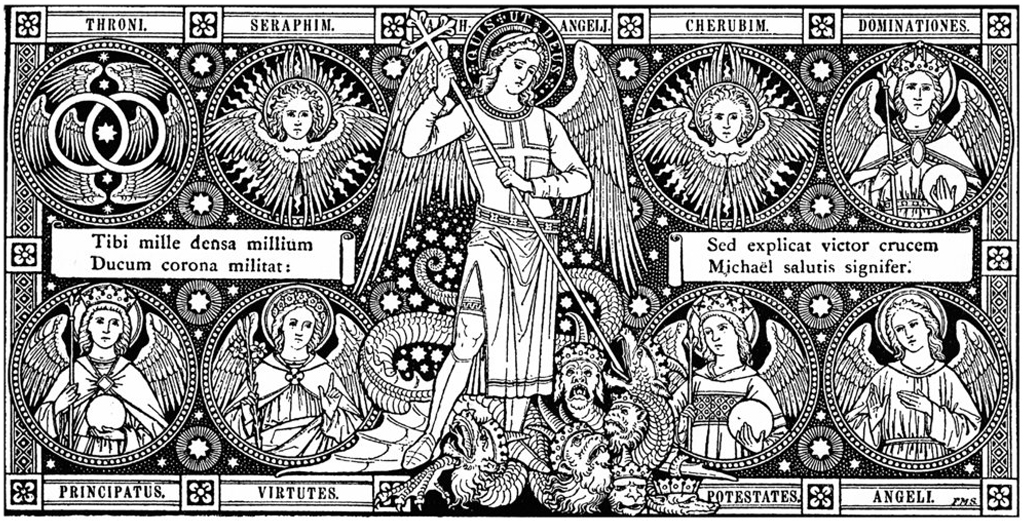
\includegraphics[width=1\textwidth,height=1\textheight,keepaspectratio]{smiguel}
\end{nscenter}

\mbox{}
\vfill
\begin{nscenter}
  Edição por Michæl, Miles Sancti Fratris Ægidii
\end{nscenter}

\end{document}